\chapter{Evaluation} \label{evaluation}

\section{Overview}

This chapter evaluates the photorealistic scene reconstruction pipeline. The pipeline is divided into two primary stages: post-processing the dataset and generating a Gaussian splat model. For testing the image post-processing script, I created a scene with challenging conditions, including high angular speeds and overexposure, to evaluate the script's ability to filter out unsuitable images. A scene recorded by the robot was used to test the Gaussian splatting and assess the 3D reconstruction quality. 

\section{Image Post-Processing Script}

To assess the effectiveness of the post-processing script, I created a dataset with simulated challenging conditions by making rapid movements and positioning a flashlight near the camera. These actions mimicked high angular speeds and overexposure, aiming to introduce blurry and overexposed frames into the dataset. Figure~\ref{fig:keyframes_before_process} shows the saved keyframe images before running the script.

\FloatBarrier
\begin{figure}[htbp]
	\centering
	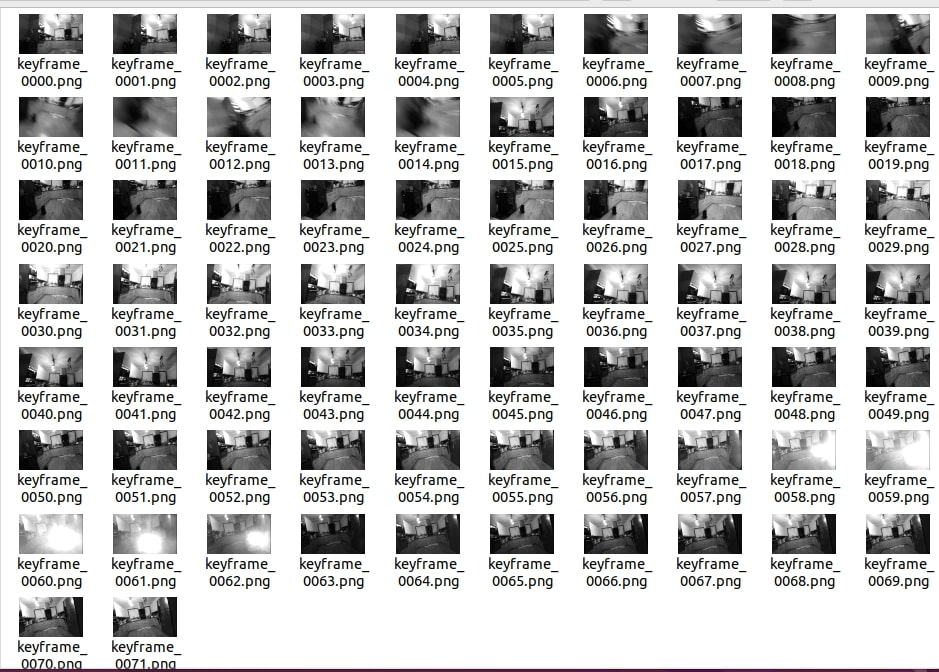
\includegraphics[width=150mm, keepaspectratio]{figures_jpg/keyframes_before_process.jpg}
	\caption{Saved images from mapping by the \textit{keyframe\_saver} node before processing}
	\label{fig:keyframes_before_process}
\end{figure}
\FloatBarrier

After running the script, which detected and removed blurry or overexposed frames, the processed image set can be seen in Figure~\ref{fig:keyframes_after_process}. The script’s output, detailing deletions and renamings, is shown in Figure~\ref{fig:image_process_script_output}. Examples of detected blurry and overexposed images that the script correctly flagged for deletion are displayed in Figure~\ref{fig:blurry_overexposed_example}.

\FloatBarrier
\begin{figure}[htbp]
	\centering
	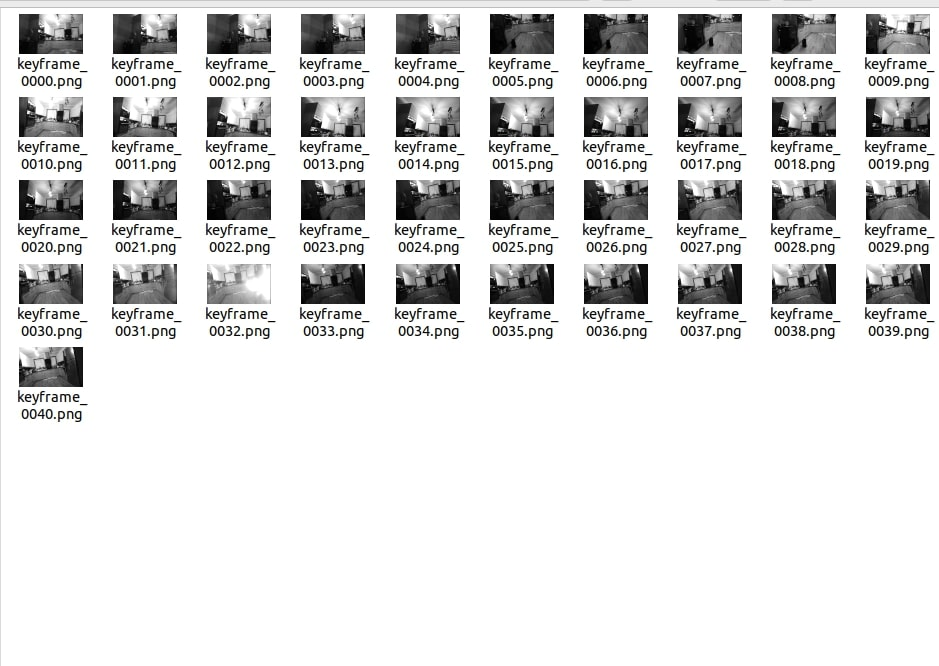
\includegraphics[width=150mm, keepaspectratio]{figures_jpg/keyframes_after_process.jpg}
	\caption{Remaining images after running the post-processing script}
	\label{fig:keyframes_after_process}
\end{figure}

\begin{figure}[htbp]
	\centering
	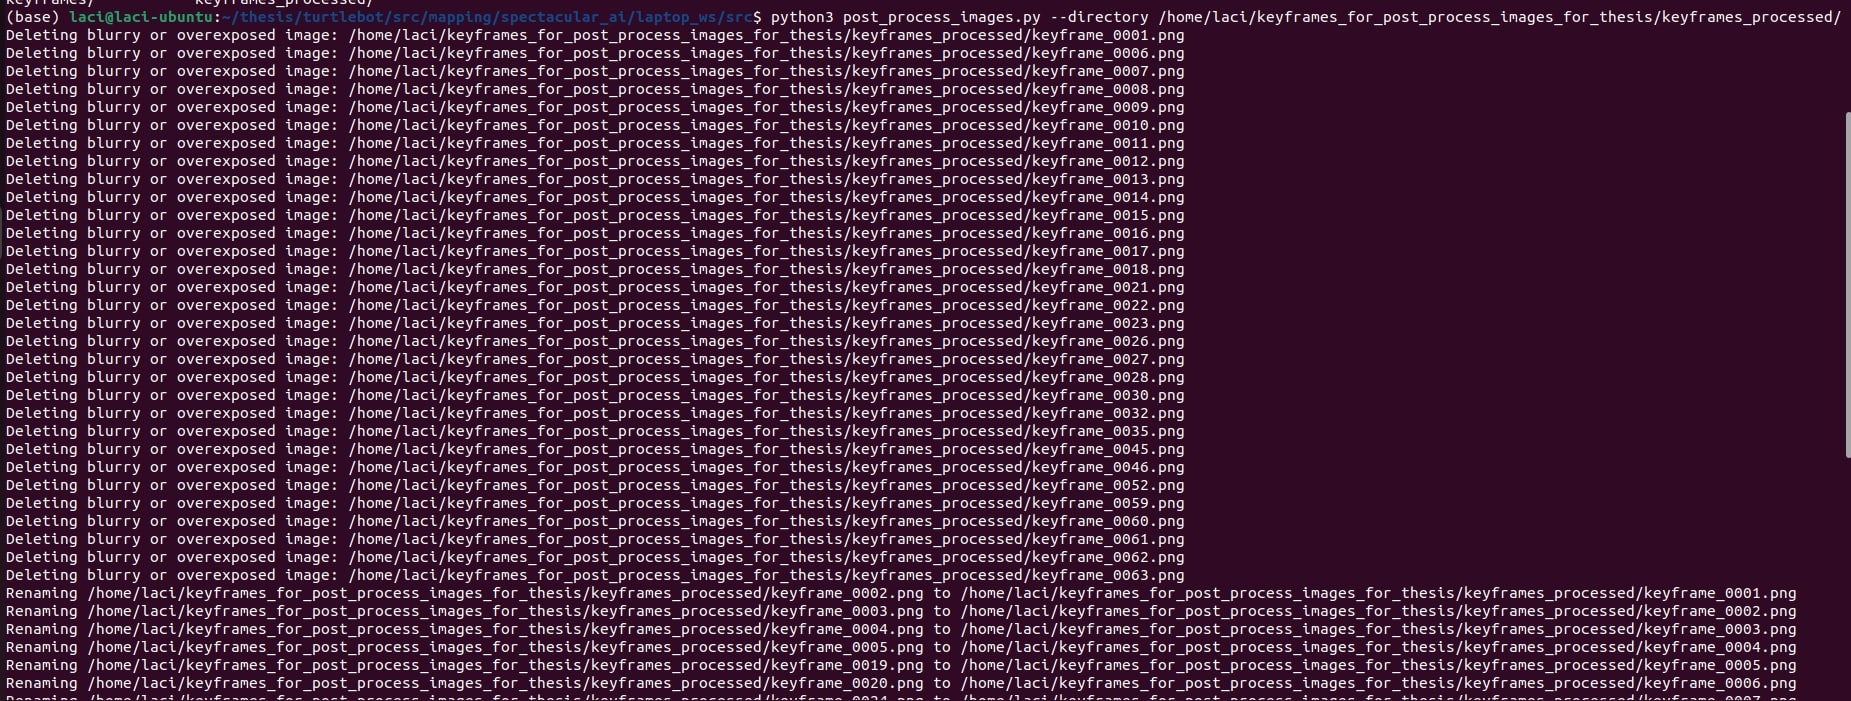
\includegraphics[width=150mm, keepaspectratio]{figures_jpg/process_script_output.jpg}
	\caption{Terminal output of the post-processing script}
	\label{fig:image_process_script_output}
\end{figure}


\begin{figure}[htbp]
	\centering
	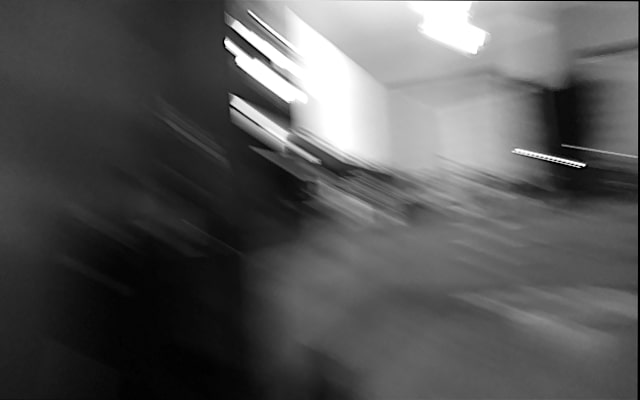
\includegraphics[width=67mm, keepaspectratio]{figures_jpg/example_for_blurry.jpg}\hspace{1cm}
	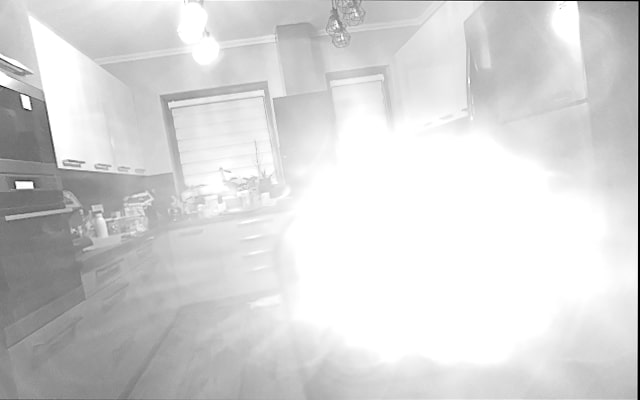
\includegraphics[width=67mm, keepaspectratio]{figures_jpg/example_for_overexposed.jpg}\\\vspace{5mm}
	\caption{Examples of blurry (left) and overexposed (right) images successfully detected and deleted by the script}
	\label{fig:blurry_overexposed_example}
\end{figure}
\FloatBarrier

I would like to note that I ran the dataset post-processing script without including the JSON files that define the poses for the keyframes. This ensures that no additional files appear in the folder shown in the figures, making the contents more straightforward and easier to interpret.

\section{Coordinate Transformations}

The output of the node that collects images and keyframe poses is shown in Figure~\ref{fig:mapping_keyframe_folder}. For each image, a corresponding JSON file is generated, containing the position and orientation of the keyframe where the image was captured. An example of such a pose file for \verb|keyframe_0012| is presented in Figure~\ref{fig:mapping_pose_json}. The images and their associated pose files share the same filename, differing only in their file extensions.

\begin{figure}[htbp]
	\centering
	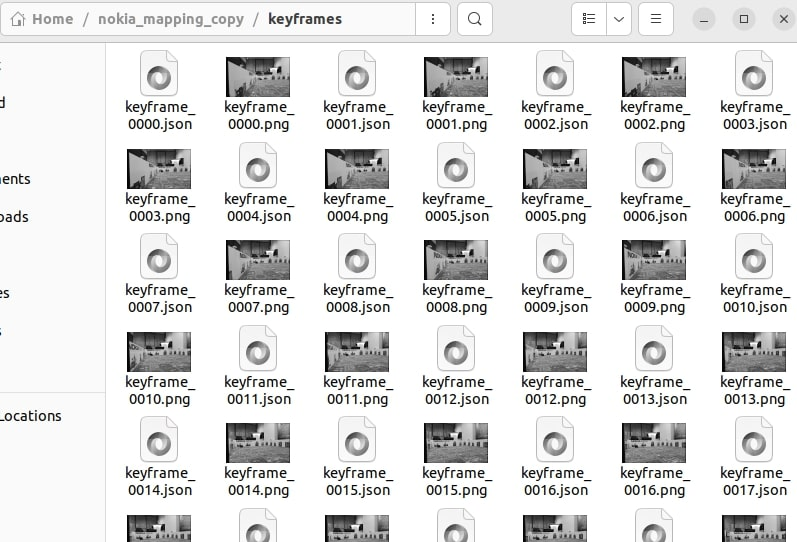
\includegraphics[width=150mm, keepaspectratio]{figures_jpg/mapping_keyframe_folder.jpg}
	\caption{Keyframe images and saved poses}
	\label{fig:mapping_keyframe_folder}
\end{figure}

\begin{figure}[htbp]
	\centering
	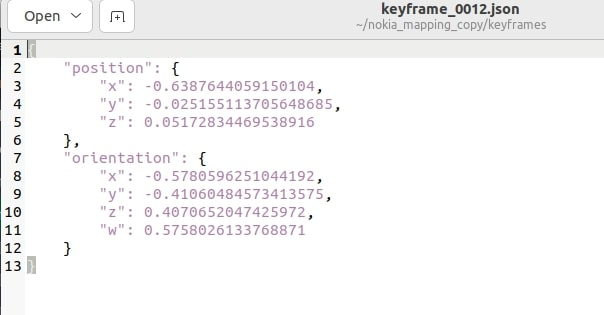
\includegraphics[width=150mm, keepaspectratio]{figures_jpg/mapping_pose_json.jpg}
	\caption{Example for pose JSON file}
	\label{fig:mapping_pose_json}
\end{figure}

Using the collected keyframes and camera intrinsic parameters, I executed my script to prepare the dataset for generating a Gaussian splat. The script processes the data, transforms the point cloud, and outputs the necessary files for the pipeline. A snapshot of the script's execution, including the progress updates for the point cloud transformation, is shown in Figure~\ref{fig:create_splatfacto_script_cli}.

\begin{figure}[htbp]
	\centering
	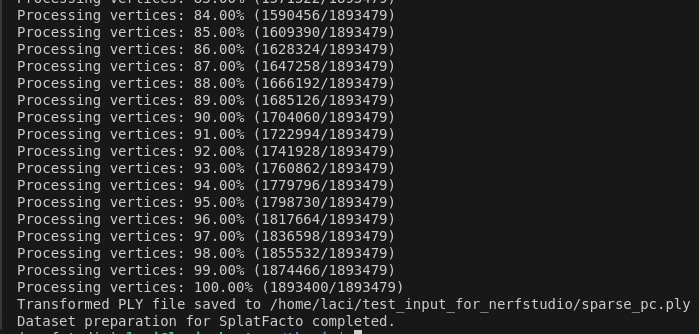
\includegraphics[width=150mm, keepaspectratio]{figures_jpg/create_splatfacto_script_cli.jpg}
	\caption{Output of the script}
	\label{fig:create_splatfacto_script_cli}
\end{figure}

The folder structure generated by the script is depicted in Figure~\ref{fig:nerfstudio_input_by_my_script}. This structure includes a folder containing the keyframe images, a transformed point cloud file, and a \verb|transforms.json| file. The \verb|transforms.json| file encodes the transformation matrices and camera intrinsics corresponding to each image's pose. A snippet of this file for \verb|keyframe_0012| is shown in Figure~\ref{fig:transforms_json}.
\begin{figure}[htbp]
	\centering
	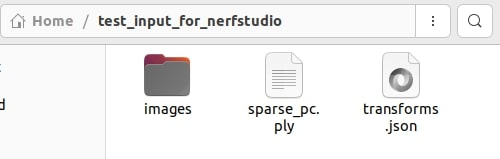
\includegraphics[width=150mm, keepaspectratio]{figures_jpg/nerfstudio_input_by_my_script.jpg}
	\caption{Created input for NeRFstudio by the script}
	\label{fig:nerfstudio_input_by_my_script}
\end{figure}

\begin{figure}[htbp]
	\centering
	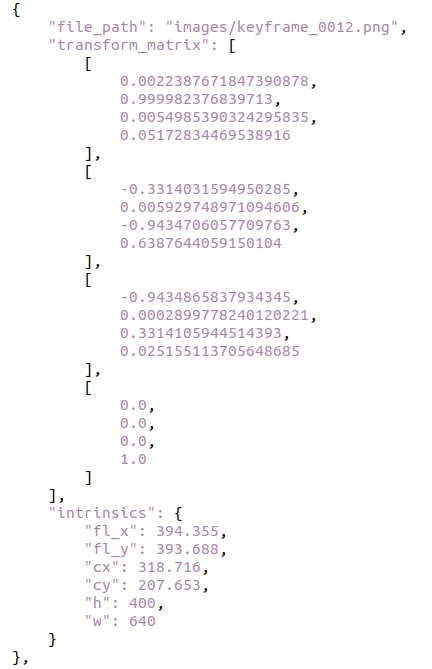
\includegraphics[width=150mm, keepaspectratio]{figures_jpg/transforms_json.jpg}
	\caption{Created transforms.json file}
	\label{fig:transforms_json}
\end{figure}

\FloatBarrier
\section{Gaussian Splatting}

To evaluate the capabilities of my pipeline and Gaussian splatting, we conducted an experiment in the Nokia office using the robot. The robot was driven within a rectangular area while the mapping node was active. During the experiment, we also started the keyframe saver and point cloud saver nodes on the laptop to capture images, their corresponding keyframe poses, and the point cloud as the robot moved. After performing image post-processing and running the dataset preparation script, we trained the \verb|splatfacto| model. The results of the reconstruction can be observed in Figure~\ref{fig:nokia_splatfacto_ours_1} and Figure~\ref{fig:nokia_splatfacto_ours_2}.

The reconstructed scene, however, was suboptimal and exhibited critical issues. While some unique features in the environment were recognizable, the overall quality was far from the desired outcome. After investigating the problem, I identified the following key observations:

\begin{itemize}
    \item Image Quality: The captured images were of sufficient quality for training the model.
    \item Pose Accuracy: The keyframe poses were accurate. To verify this, we manually measured the distances and rotations between distant keyframes and compared them with the pose data provided by the camera, finding a strong correlation.
    \item Transformation Validation: The transformations were verified during training by inspecting the keyframe trajectory in the viewer. The trajectory accurately reflected the robot's real-world movements. Additionally, the viewer allowed us to display the point cloud during training, which confirmed proper alignment between the poses and the point cloud. This alignment is evident in Figure~\ref{fig:trajectory_and_pointcloud} and Figure~\ref{fig:pointcloud_debug}, where both the trajectory and point cloud depict the same corner of the environment.
    \item Point Cloud Issues: The primary cause of the suboptimal results was the point cloud itself. As seen in Figure~\ref{fig:pointcloud_debug}, the point cloud contained a significant amount of noise—points that do not exist in the real environment. This noise severely impacted the reconstruction, as Gaussian splatting is highly sensitive to such artifacts. Since Gaussian splatting fits a Gaussian to each point, even noise points contribute to the reconstruction as surfaces. Additionally, there was a bump in the floor, causing certain floor points to be slightly tilted, as illustrated in Figure~\ref{fig:pointcloud_debug1}.
\end{itemize}

\begin{figure}[htbp]
	\centering
	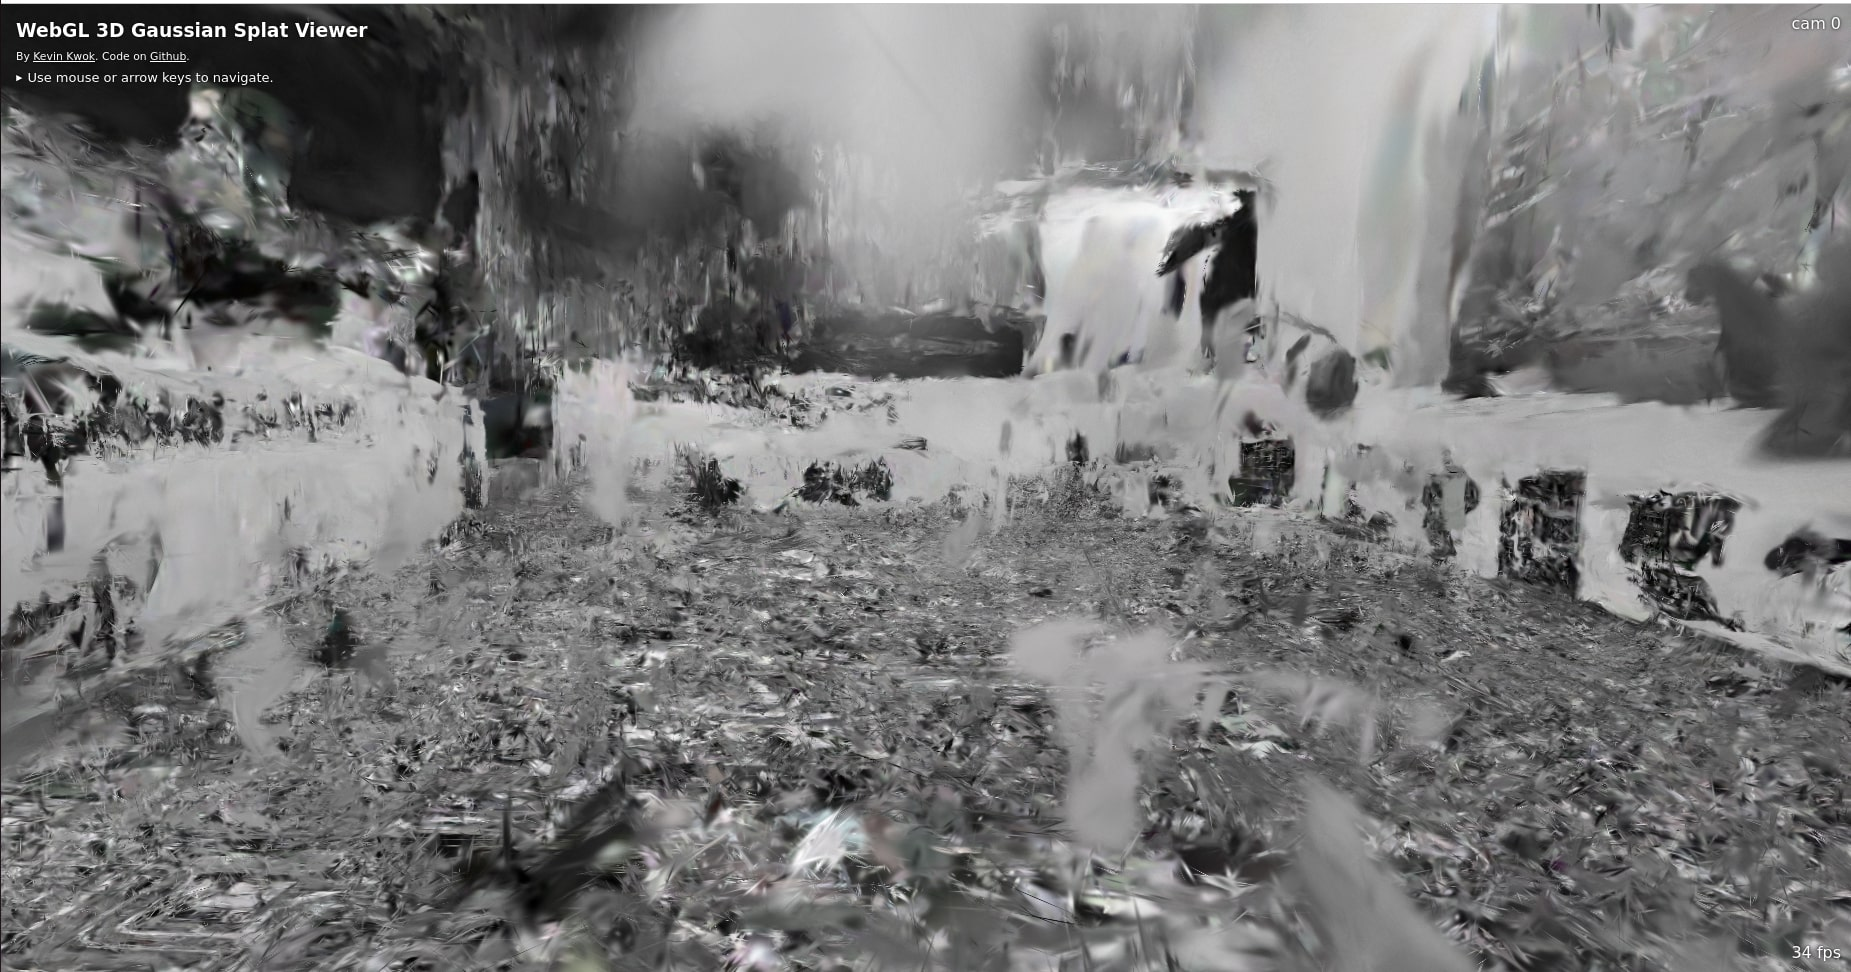
\includegraphics[width=150mm, keepaspectratio]{figures_jpg/nokia_splatfacto_ours1.jpg}
	\caption{Reconstructed map in the Nokia office with the \textit{splatfacto} model}
	\label{fig:nokia_splatfacto_ours_1}
\end{figure}

\begin{figure}[htbp]
	\centering
	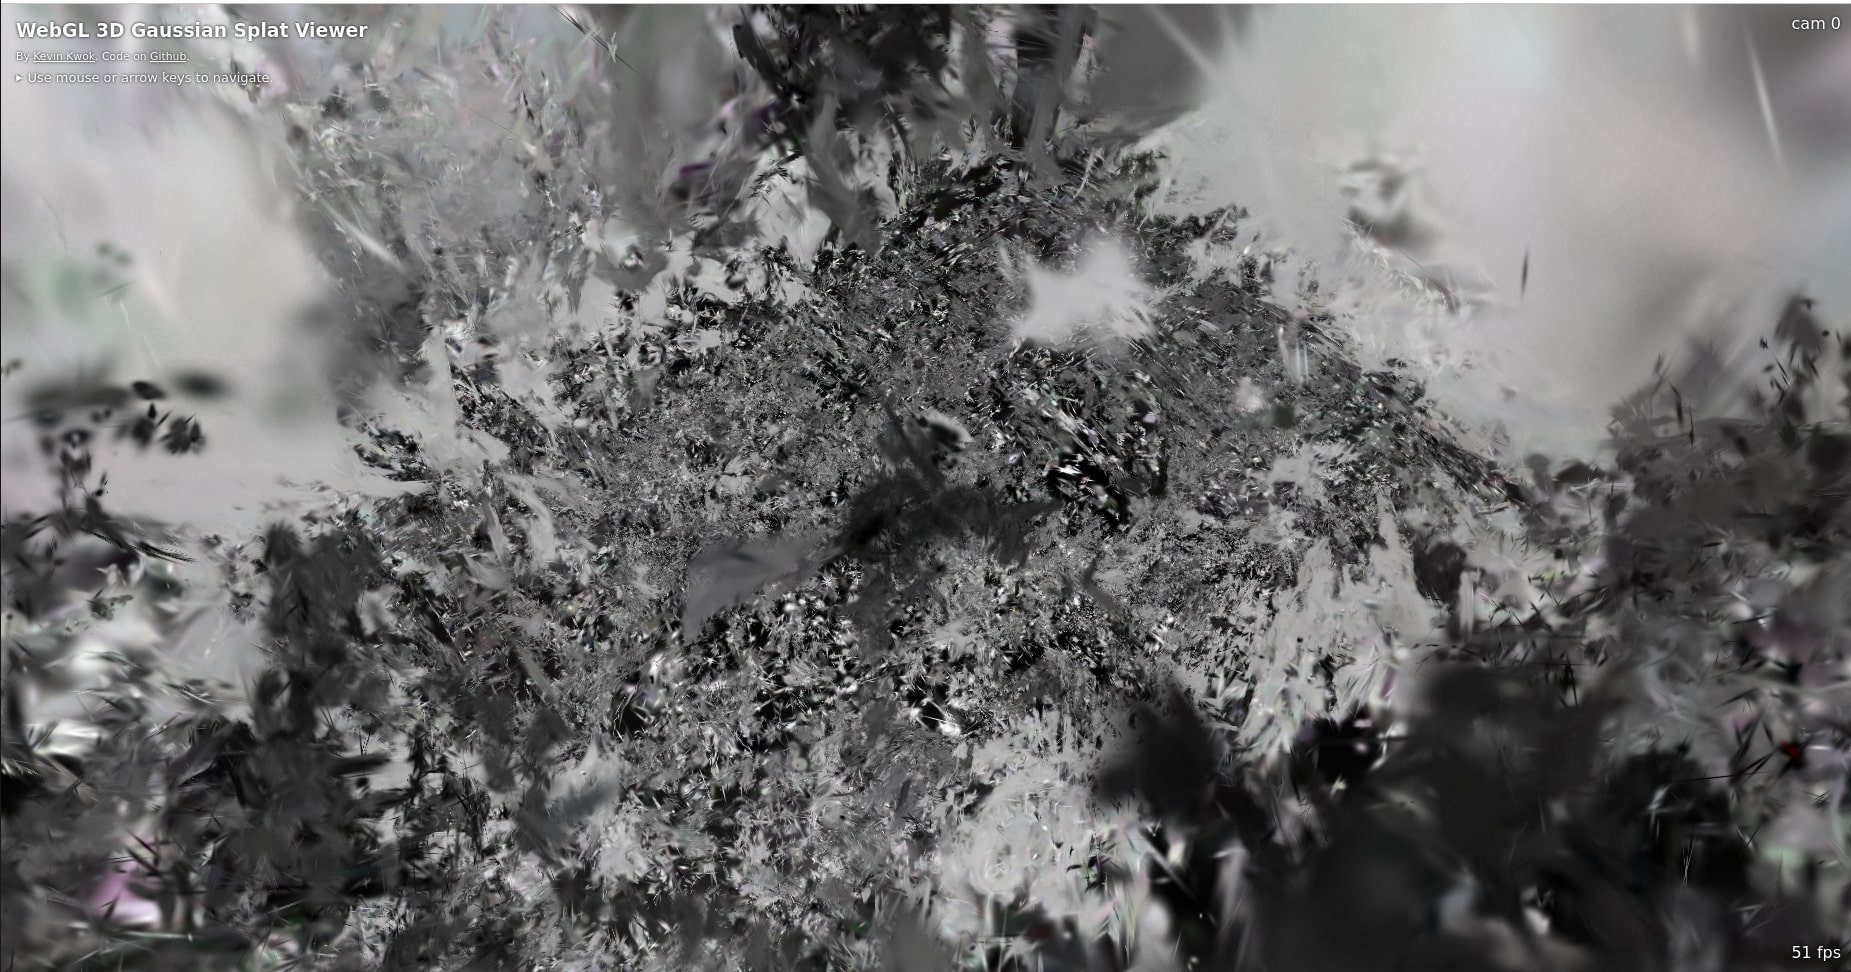
\includegraphics[width=150mm, keepaspectratio]{figures_jpg/nokia_splatfacto_ours2.jpg}
	\caption{Reconstructed map in the Nokia office with the \textit{splatfacto} model}
	\label{fig:nokia_splatfacto_ours_2}
\end{figure}

\begin{figure}[htbp]
	\centering
	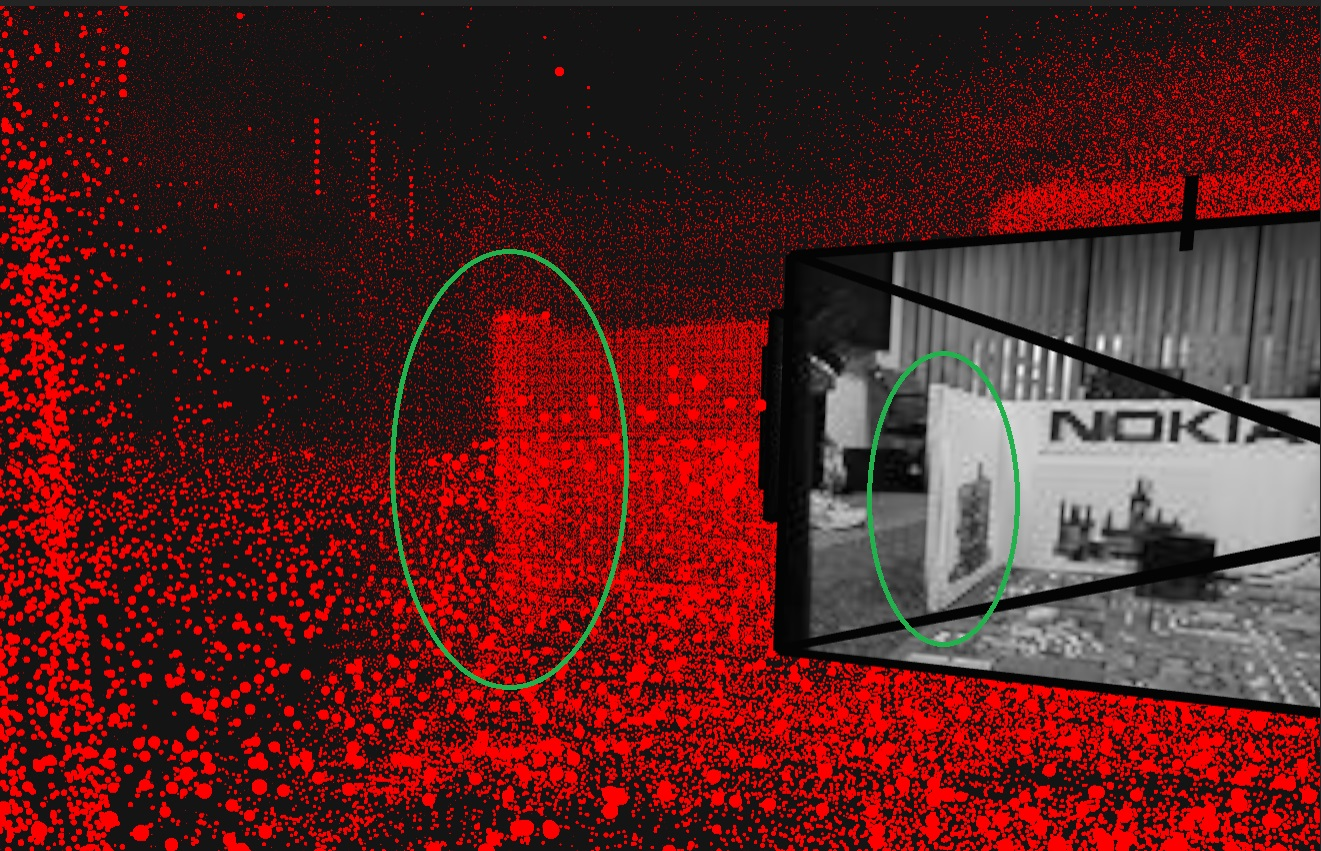
\includegraphics[width=150mm, keepaspectratio]{figures_jpg/trajectory_and_pointcloud_debug.jpg}
	\caption{Reconstructed map in the Nokia office with the \textit{splatfacto} model}
	\label{fig:trajectory_and_pointcloud}
\end{figure}

\begin{figure}[htbp]
	\centering
	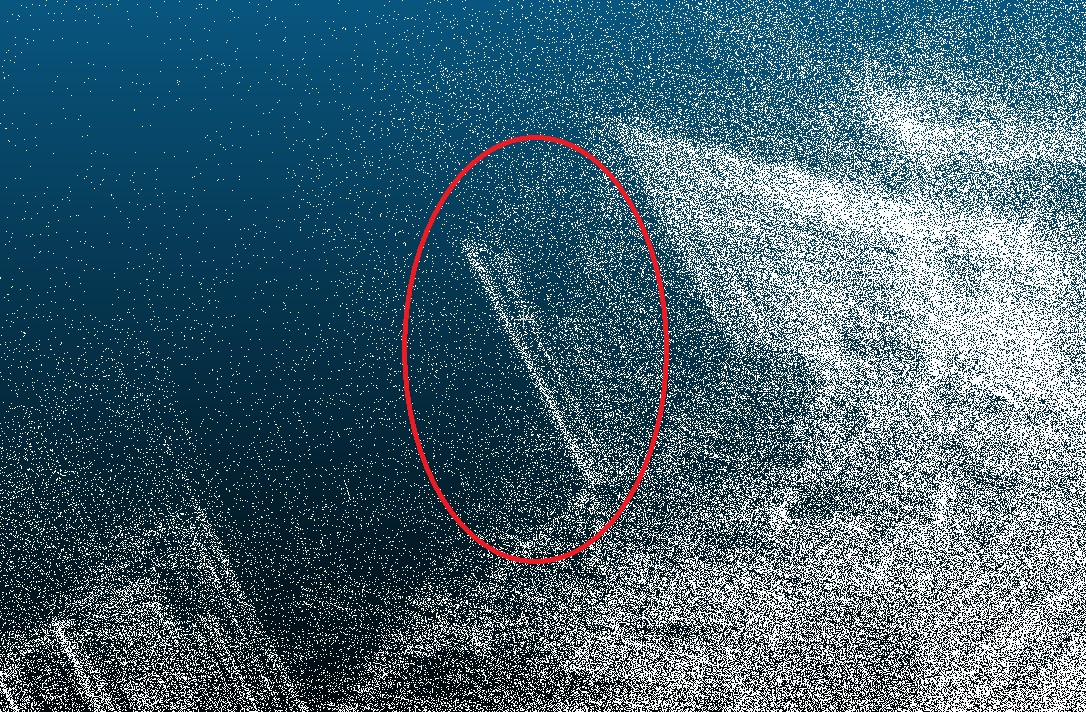
\includegraphics[width=150mm, keepaspectratio]{figures_jpg/pointcloud_debug.jpg}
	\caption{Reconstructed map in the Nokia office with the \textit{splatfacto} model}
	\label{fig:pointcloud_debug}
\end{figure}

\begin{figure}[htbp]
	\centering
	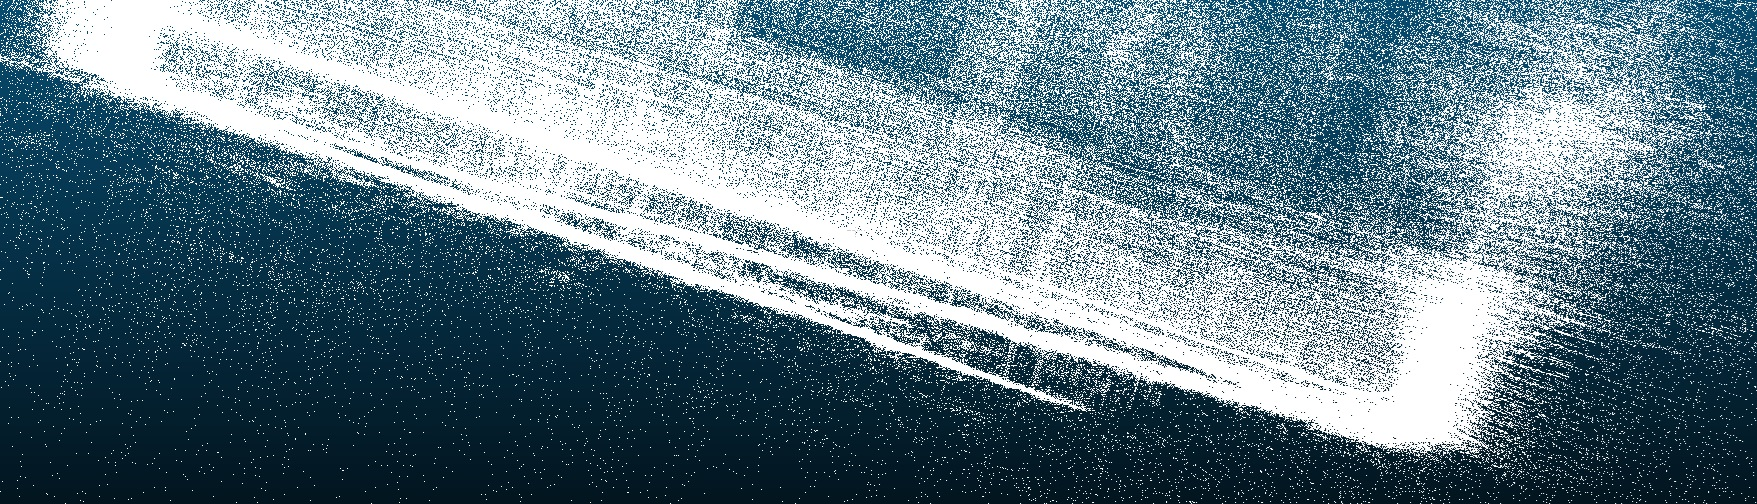
\includegraphics[width=150mm, keepaspectratio]{figures_jpg/pointcloud_debug1.jpg}
	\caption{Reconstructed map in the Nokia office with the \textit{splatfacto} model}
	\label{fig:pointcloud_debug1}
\end{figure}


To validate the usability of the reconstruction for mapping scenarios, we compared our results with those produced by COLMAP, a tool for point cloud reconstruction and pose estimation from images. The COLMAP-generated reconstruction is shown in Figure~\ref{fig:nokia_splatfacto_colmap_1} and Figure~\ref{fig:nokia_splatfacto_colmap_2}. The training process can be observed on a video\footnote{\url{https://youtu.be/qfDjOSoVy9Y}}.

\begin{figure}[htbp]
	\centering
	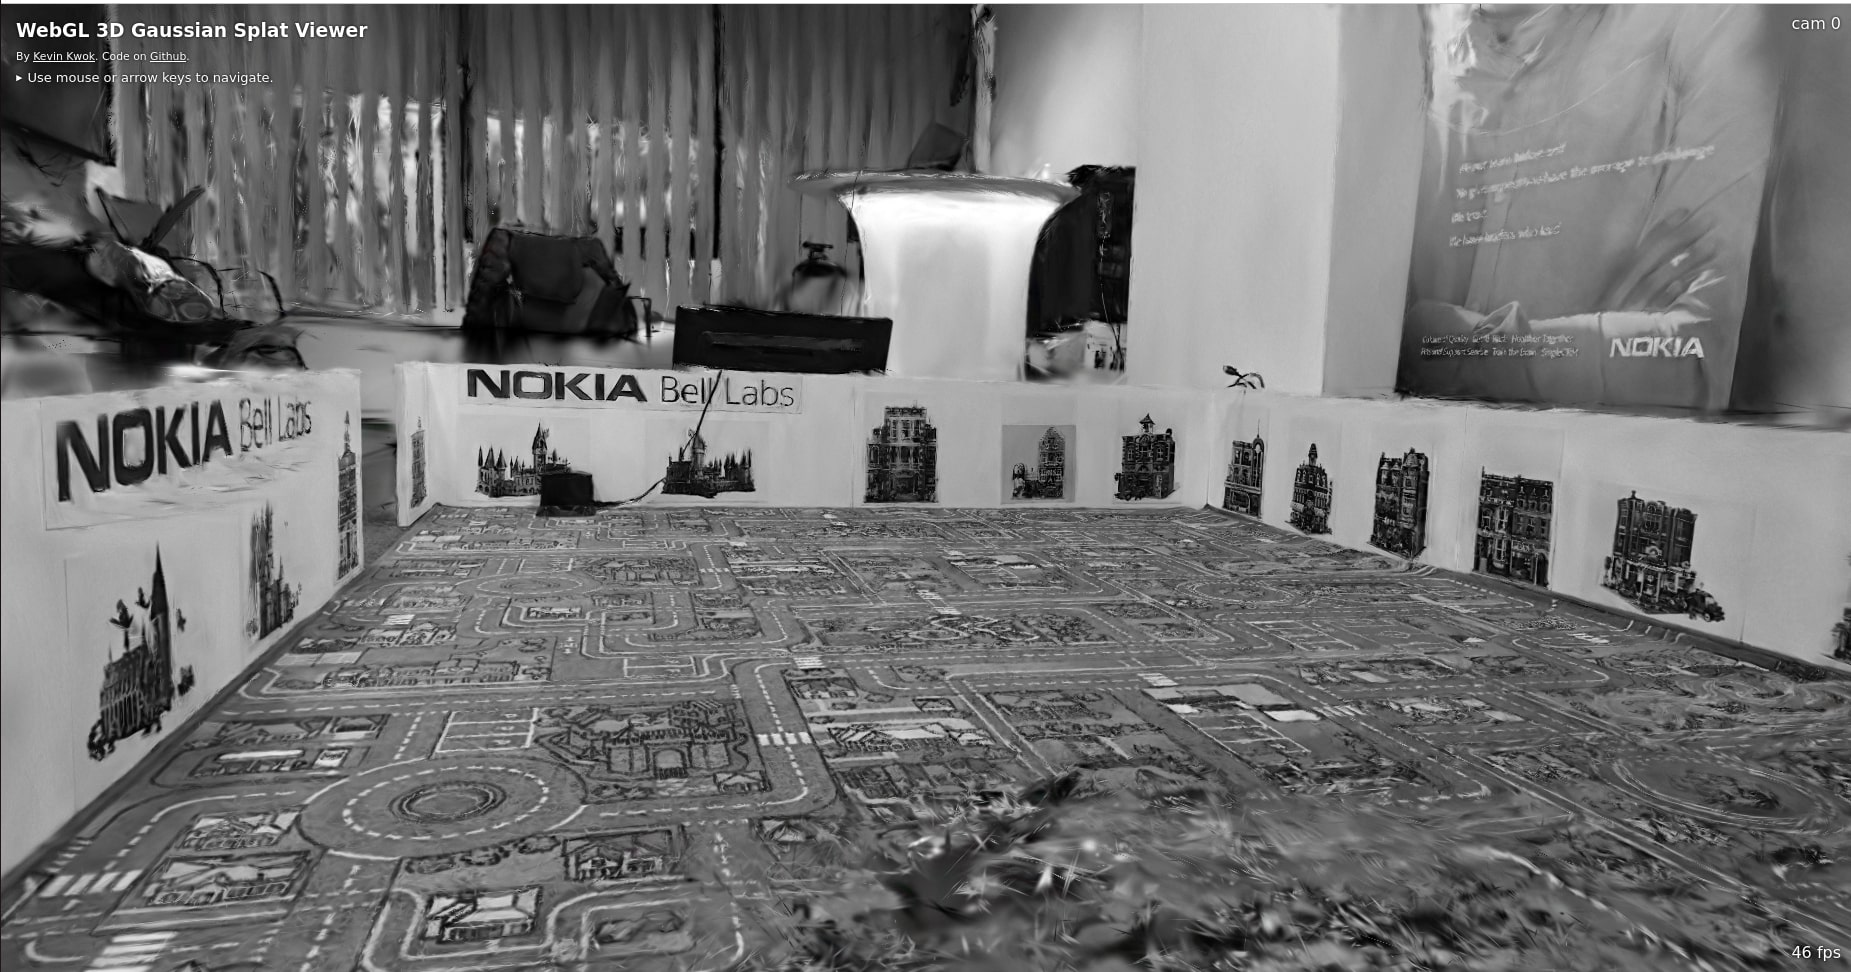
\includegraphics[width=150mm, keepaspectratio]{figures_jpg/nokia_splatfacto_1.jpg}
	\caption{Reconstructed map in the Nokia office with the \textit{splatfacto} model}
	\label{fig:nokia_splatfacto_colmap_1}
\end{figure}

\begin{figure}[htbp]
	\centering
	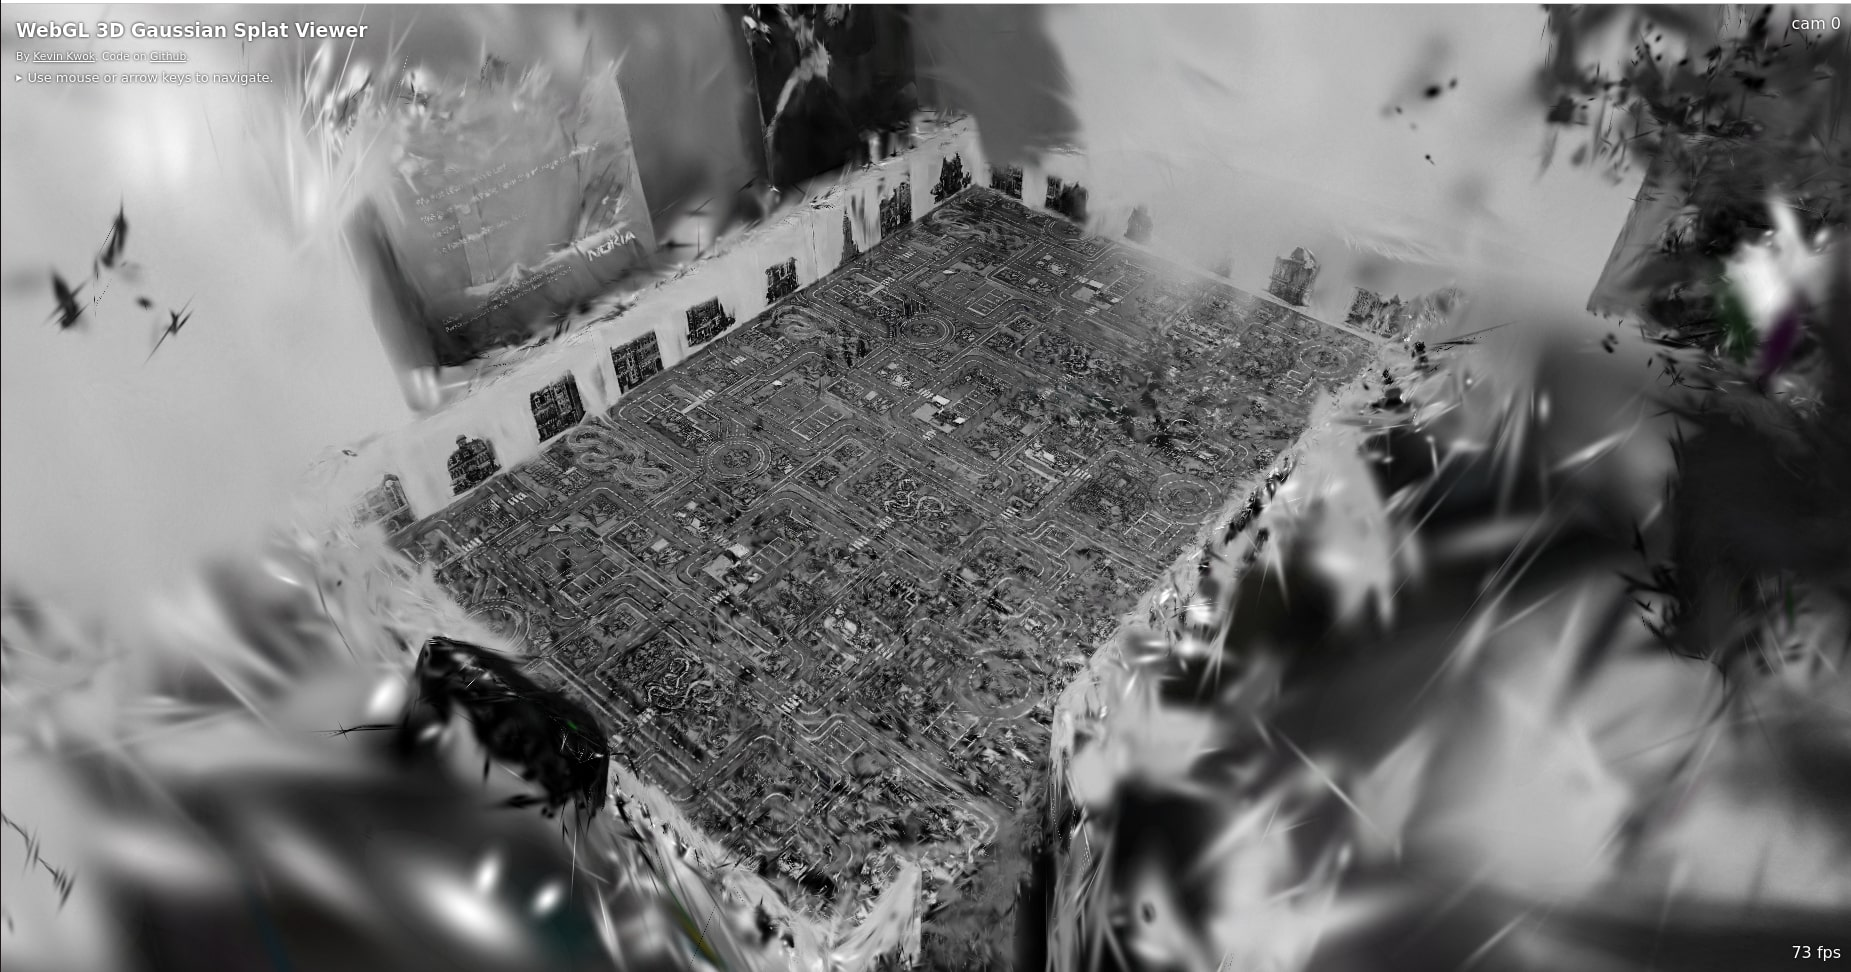
\includegraphics[width=150mm, keepaspectratio]{figures_jpg/nokia_splatfacto_2.jpg}
	\caption{Reconstructed map in the Nokia office with the \textit{splatfacto} model}
	\label{fig:nokia_splatfacto_colmap_2}
\end{figure}

In conclusion, the reconstruction obtained using COLMAP accurately depicts the real environment. If the noise in the camera-generated point cloud could be effectively filtered, the results from our pipeline could potentially match or even exceed COLMAP's accuracy. Unfortunately, due to time constraints, implementing such a filtering mechanism was beyond the scope of this thesis.
